\chapter{مقدمه}


بیشتر سرویس‌های شبکه بر روی سخت افزارهای اختصاصی به نام
\lr{middle box}
ساخته می‌شوند.
تنوع و تعداد رو به افزایش سرویس‌های جدیدی که توسط کاربران تقاضا می‌گردد
باعث هزینه‌های زیاد برای خرید و نگهداری
\lr{middle box}‌ها
توسط اپراتورها شده است.
به تازگی فراهم آورندگان شبکه
شروع به حرکت به سوی مجازی‌سازی و نرم‌افزاری کردن بسترهای شکبه کرده‌اند،
به این ترتیب آن‌ها قادر خواهند بود
سرویس‌های نوآورانه‌ای به کاربران ارائه بدهند.

مجازی‌سازی توابع شبکه‌ راهکاری است که برای همین منظور پیشنهاد شده است.
مجازی‌سازی توابع شبکه‌ در واقع راه‌حل‌های مشخصی را برای چالش‌های جای‌گذاری،
زنجیره‌سازی و هماهنگی سرویس‌های شبکه فراهم می‌آورد.

ایده‌ی اصلی مجازی‌سازی توابع شبکه جداسازی تجهیزات فیزیکی شبکه از کارکردهایی می‌باشد که
بر روی آن‌ها اجرا می‌شوند.
به این معنی که یک کاکرد شبکه مانند دیوار آتش می‌تواند بر روی یک
\lr{TSP}
به عنوان یک نرم‌افزار ساده فرستاده شود.
با این روش یک سرویس می‌تواند به مجموعه‌ای از کارکردهای مجازی شبکه‌ای که می‌توانند به صورت نرم‌افزاری پیاده‌سازی شده
و روی یک یا تعداد سرور استاندارد فیزیکی اجرا شوند، شکسته شود.
کارکرهای مجازی شبکه‌ای می‌توانند در مکان‌های مختلف بازمکان‌یابی یا نمونه‌سازی شوند بدون آنکه
نیاز به خریداری و نصب تجهیز جدیدی باشد.
\cite{Mijumbi2016}

\section{معماری \lr{NFV}}
با توجه به استاندارد \lr{ETSI} معماری \lr{NFV}
از سه عنصر کلیدی تشکیل شده است.
زیرساخت مجازی‌سازی کارکردهای شبکه،
کارکردهای مجازی شبکه‌ای و
\lr{NFV MANO}.
این اجزا در شکل \cref{fig.1} نمایش داده شده‌اند.

\begin{figure}[!h]
\center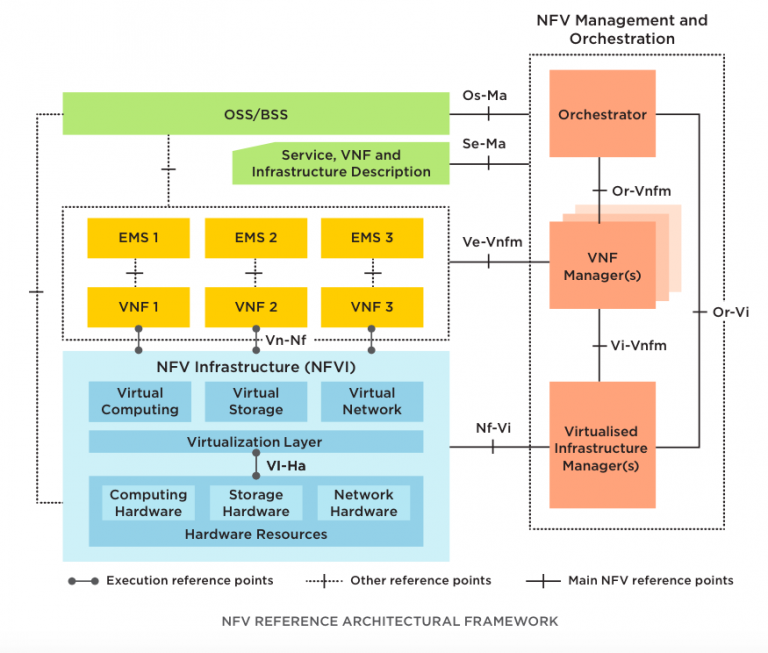
\includegraphics[scale=.6]{images/nfv-arch}
\caption{معماری مجازی‌سازی کارکردهای شبکه
\cite{Mijumbi2016}
}\label{fig.1}
\end{figure}

\subsection{زیرساخت مجازی‌سازی کارکردهای شبکه}
زیرساخت مجازی‌سازی کارکردهای شبکه ترکیبی از منابع نرم‌افزاری و سخت‌افزاری می‌باشد
که محیطی برای نصب
کارکردهای مجازی شبکه فراهم می‌آورد.

منابع سخت‌افزاری شامل سخت‌افزارهای محاسباتی بدون اختصاصی‌سازی،
ذخیره‌سازها و شبکه
(شامل لینک‌ها و گره‌ها)
می‌باشند
که پردازش، ذخیره‌سازی و ارتباط را
برای کارکردهای مجازی شبکه فراهم می‌آورند.
منابع مجازی انتزاعی از منابع شبکه‌ای، پردازشی و ذخیر‌ه‌سازی هستند.
این انتزاع از طریق لایه‌ی مجازی‌سازی (بر پایه‌ی \lr{hypervisor}) ایجاد می‌شود،
که منابع مجازی را از منابع فیزیکی جدا می‌کند.

در مراکز داده‌ای ممکن است منابع پردازشی و ذخیره‌سازی تحت عنوان یک یا چند
ماشین مجازی نمایش داده شوند در حالی که شبکه‌های مجازی از لینک‌ها و گره‌های مجازی تشکیل می‌شوند.
یک گره‌ی مجازی یک جز نرم‌افزاری با قابلیت مسیریابی یا میزبانی می‌باشد.

\subsection{کاکردهای مجازی شبکه‌ای}
یک کارکرد شبکه، یک بلوک عملیاتی در زیرساخت شبکه است که عملکرد رفتاری و رابط‌های ارتباط با خارج خوش تعریف دارد.
مثال‌هایی از کاکردهای شبکه می‌تواند شامل
\lr{DHCP}
یا
\lr{firewall}
و ... باشد.
با این توضیحات کاکرد مجازی شبکه، پیاده‌سازی یک کارکرد شبکه می‌باشد
که می‌تواند روی منابع مجازی مانند ماشین مجازی اجرا شود.